\documentclass[12pt, oneside]{book}
\usepackage[a4paper,top=2.5cm,bottom=2.5cm,left=3.5cm,right=2cm]{geometry}
\usepackage[utf8]{inputenc}
\usepackage[T1]{fontenc}
\usepackage{graphicx}
\usepackage{url}
\usepackage[slovak]{babel} % vypnite pre prace v anglictine
\linespread{1.25} % hodnota 1.25 by mala zodpovedat 1.5 riadkovaniu
\usepackage{tabularx}


\usepackage{fancyhdr}



% -------------------
% --- Definicia zakladnych pojmov
% --- Vyplnte podla vasho zadania
% -------------------
\def\mfrok{2016}
\def\mfnazov{Workflow management rolí a užívateľov}
\def\mftyp{Bakalárska práca}
\def\mfautor{Pavol Martiš}
\def\mfskolitel{prof. RNDr. Gabriel Juhás, PhD.}
\def\mfevidenceneCislo{FEI-5382-72557}

%ak mate konzultanta, odkomentujte aj jeho meno na titulnom liste
\def\mfkonzultant{tit. Meno Priezvisko, tit. }  

\def\mfmiesto{Bratislava, \mfrok}

%aj cislo odboru je povinne a je podla studijneho odboru autora prace
\def\mfodbor{ 9.2.9 aplikovaná informatika } 
\def\program{ Aplikovaná informatika }
\def\mfpracovisko{ Ústav informatiky a matematiky }




%moje funkcie 
\newcommand{\mychapter}[2]{
	\setcounter{chapter}{#1}
	\setcounter{section}{0}
	\chapter*{#2}
	\addcontentsline{toc}{chapter}{#2}
}

\begin{document}     

% -------------------
% --- Obalka ------
% -------------------
\thispagestyle{empty}

\begin{center}
\sc\large
Slovenská technická univerzita
\\*Fakulta elektrotechniky a informatiky\\
\end{center}


{	
	Evidenčné číslo: \mfevidenceneCislo
	\noindent 
}

\vfill
\begin{center}
{\LARGE\mfnazov}\\
\Large\mftyp
\end{center}

\vfill

{\sc\large 
\noindent \mfrok\\
\mfautor
}

\eject % EOP i
% --- koniec obalky ----

% -------------------
% --- Titulný list
% -------------------

\thispagestyle{empty}
\noindent

\begin{center}
\sc  
\large
Slovenská technická univerzita v Bratislave\\
Fakulta elektrotechniky a informatiky\\
\end{center}
\begin{tabular}{ll}
Evidenčné číslo: \mfevidenceneCislo
\end{tabular}

\vfill

\begin{center}
{\LARGE\mfnazov}\\
\Large \mftyp
\end{center}

\vfill

\noindent
\begin{tabular}{ll}
Študijný program: & \program \\
Študijný odbor: & \mfodbor \\
Školiace pracovisko: & \mfpracovisko \\
Školiteľ: & \mfskolitel \\
% Konzultant: & \mfkonzultant \\
\end{tabular}

\vfill


\noindent \mfmiesto\\
\mfautor

\eject % EOP i


% --- Koniec titulnej strany


% -------------------
% --- Zadanie z AIS
% -------------------
% v tlačenej verzii s podpismi zainteresovaných osôb.
% v elektronickej verzii sa zverejňuje zadanie bez podpisov

\newpage 
\thispagestyle{empty}
\hspace{-2cm}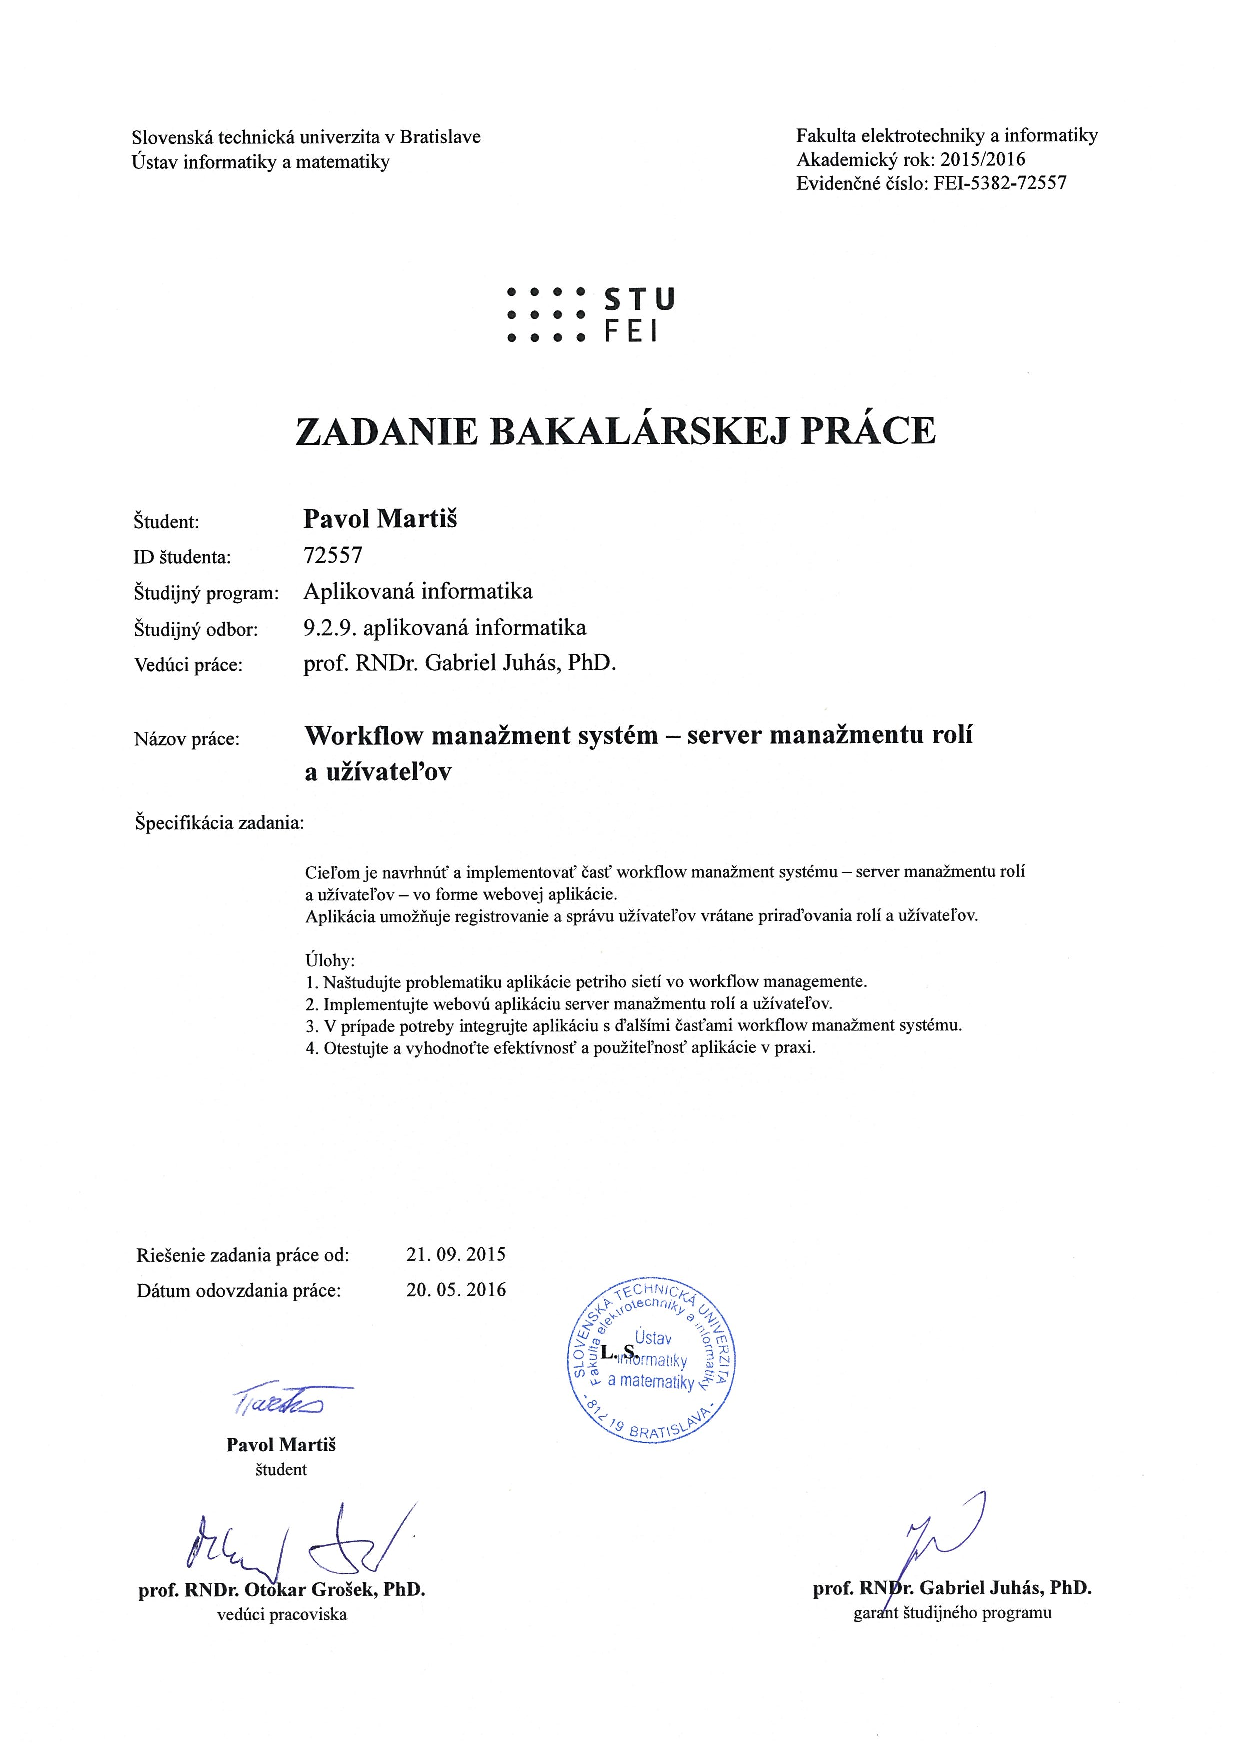
\includegraphics[width=1.1\textwidth]{images/zadanie}

% --- Koniec zadania

\frontmatter

% -------------------
%   Poďakovanie - nepovinné
% -------------------
\setcounter{page}{3}
\newpage 
\begin{center}
	\bf Poďakovanie: \\
\end{center}

\noindent  

\vfill


% --- Koniec poďakovania

% -------------------
%   Abstrakt - Slovensky
% -------------------
\newpage 
\section*{Abstrakt}


Slovenský abstrakt v rozsahu 100-500 slov, jeden odstavec. Abstrakt
stručne sumarizuje výsledky práce. Mal by byť pochopiteľný pre bežného
informatika. Nemal by teda využívať skratky, termíny alebo označenie
zavedené v práci, okrem tých, ktoré sú všeobecne známe.

\paragraph*{Kľúčové slová:} užívateľ, rola , workflow, Petriho sieť, RBAC , workflow
% --- Koniec Abstrakt - Slovensky


% -------------------
% --- Abstrakt - Anglicky 
% -------------------
\newpage 
\section*{Abstract}

Abstract in the English language (translation of the abstract in the
Slovak language).


\paragraph*{Keywords:} 

% --- Koniec Abstrakt - Anglicky

% -------------------
% --- Predhovor - v informatike sa zvacsa nepouziva
% -------------------
%\newpage 
%\thispagestyle{empty}
%
%\huge{Predhovor}
%\normalsize
%\newline
%Predhovor je všeobecná informácia o práci, obsahuje hlavnú charakteristiku práce 
%a okolnosti jej vzniku. Autor zdôvodní výber témy, stručne informuje o cieľoch 
%a význame práce, spomenie domáci a zahraničný kontext, komu je práca určená, 
%použité metódy, stav poznania; autor stručne charakterizuje svoj prístup a svoje 
%hľadisko. 
%
% --- Koniec Predhovor


% -------------------
% --- Obsah
% -------------------

\newpage 


\tableofcontents



% ---  Koniec Obsahu

% -------------------
% --- Zoznamy tabuliek, obrázkov - nepovinne
% -------------------

\newpage 

{\LARGE Zoznam skratiek}\\

\noindent
WFMS – Workflow management system\\
RBAC – Role-based access control\\
CSS - Cascading Style Sheets\\
XML - Extensible Markup Language\\



\listoffigures



% ---  Koniec Zoznamov

\mainmatter


\input uvod.tex 

\input analyza.tex

\input opis.tex

\input zaver.tex

% -------------------
% --- Bibliografia
% -------------------


\newpage

\backmatter

\thispagestyle{empty}
\nocite{*}
\clearpage

\bibliographystyle{plain}

\bibliography{literatura} 

%Prípadne môžete napísať literatúru priamo tu
\begin{thebibliography}{5}
 
\bibitem{gabova_kniha} MOLINA H. G. - ULLMAN J. D. - WIDOM J., 2002, Database Systems, Upper Saddle River : Prentice-Hall, 2002, 1119 s., Pearson International edition, 0-13-098043-9


\end{thebibliography}

%---koniec Referencii

% -------------------
%--- Prilohy---
% -------------------

%Nepovinná časť prílohy obsahuje materiály, ktoré neboli zaradené priamo  do textu. Každá príloha sa začína na novej strane.
%Zoznam príloh je súčasťou obsahu.
%
%\addcontentsline{toc}{chapter}{Appendix A}
%\input AppendixA.tex
%
%\addcontentsline{toc}{chapter}{Appendix B}
%\input AppendixB.tex


\end{document}






